%-----------------------------------------------------------------------
%
%   UFRJ  - Universidade Federal do Rio de Janeiro
%   COPPE - Coordenação dos Programas de Pós-graduação em Engenharia
%   PEE   - Programa de Engenharia Elétrica
%
%
%   Projeto EMMA - 
%
%                                                        19/out/15, Rio
%                                                        Estevão F. Ferrão
%----------------------------------------------------------------------
%
%  Compilar usando PDFLaTeX
%
%----------------------------------------------------------------------
\documentclass[12pt,a4paper]{article}
\usepackage{macros/ROSApackages} 
 
%-----------------------------------------------------------------------
%
%   UFRJ  - Universidade Federal do Rio de Janeiro
%   COPPE - Coordena��o dos Programas de P�s-gradua��o em Engenharia
%   PEE   - Programa de Engenharia El�trica
%
%
%   Projeto ROSA - Rob� para opera��o de stoplogs alagados
%
%   Settings
%                                                         Ramon R. Costa
%                                                         20/mar/14, Rio
%-----------------------------------------------------------------------

%---------------------------------------------------------- COLORS -----
%--------------------------------------------------- Bright colors -----
\definecolor{brightred}     {rgb}{1.00, 0.95, 0.95}
\definecolor{brightgreen}   {rgb}{0.95, 1.00, 0.95}
\definecolor{brightblue}    {rgb}{0.95, 0.95, 1.00}

\definecolor{brightyellow}  {rgb}{1.00, 1.00, 0.95}
\definecolor{brightmagenta} {rgb}{1.00, 0.95, 1.00}
\definecolor{brightcyan}    {rgb}{0.95, 1.00, 1.00}

\definecolor{brightorange}  {rgb}{1.00, 0.95, 0.85}

%----------------------------------------------------- Pale colors -----
\definecolor{palered}     {rgb}{1.00, 0.85, 0.85}
\definecolor{palegreen}   {rgb}{0.85, 1.00, 0.85}
\definecolor{paleblue}    {rgb}{0.85, 0.85, 1.00}

\definecolor{paleyellow}  {rgb}{1.00, 1.00, 0.85}
\definecolor{palemagenta} {rgb}{1.00, 0.85, 1.00}
\definecolor{palecyan}    {rgb}{0.85, 1.00, 1.00}

\definecolor{paleorange}  {rgb}{1.00, 0.85, 0.65}

%---------------------------------------------------- Light colors -----
\definecolor{lightred}     {rgb}{0.95, 0.00, 0.00}
\definecolor{lightgreen}   {rgb}{0.00, 0.95, 0.00}
\definecolor{lightblue}    {rgb}{0.00, 0.00, 0.95}

\definecolor{lightyellow}  {rgb}{0.95, 0.95, 0.00}
\definecolor{lightmagenta} {rgb}{0.95, 0.00, 0.95}
\definecolor{lightcyan}    {rgb}{0.00, 0.95, 0.95}

\definecolor{lightgray}    {rgb}{0.95, 0.95, 0.95}

\definecolor{lightorange}  {rgb}{0.95, 0.63, 0.00}

%--------------------------------------------------- Middle colors -----
\definecolor{midred}     {rgb}{0.85, 0.00, 0.00}
\definecolor{midgreen}   {rgb}{0.00, 0.85, 0.00}
\definecolor{midblue}    {rgb}{0.00, 0.00, 0.85}

\definecolor{midyellow}  {rgb}{0.85, 0.85, 0.00}
\definecolor{midmagenta} {rgb}{0.85, 0.00, 0.85}
\definecolor{midcyan}    {rgb}{0.00, 0.85, 0.85}

\definecolor{midgray}    {rgb}{0.85, 0.85, 0.85}

\definecolor{midorange}  {rgb}{0.85, 0.57, 0.00}

%--------------------------------------------------- Normal colors -----
\definecolor{red}     {rgb}{0.75, 0.00, 0.00}
\definecolor{green}   {rgb}{0.00, 0.75, 0.00}
\definecolor{blue}    {rgb}{0.00, 0.00, 0.75}

\definecolor{yellow}  {rgb}{0.75, 0.75, 0.00}
\definecolor{magenta} {rgb}{0.75, 0.00, 0.75}
\definecolor{cyan}    {rgb}{0.00, 0.75, 0.75}

\definecolor{gray}    {rgb}{0.75, 0.75, 0.75}

\definecolor{orange}  {rgb}{0.75, 0.50, 0.00}

%--------------------------------------------------- Shadow colors -----
\definecolor{shadred}     {rgb}{0.65, 0.00, 0.00}
\definecolor{shadgreen}   {rgb}{0.00, 0.65, 0.00}
\definecolor{shadblue}    {rgb}{0.00, 0.00, 0.65}

\definecolor{shadyellow}  {rgb}{0.65, 0.65, 0.00}
\definecolor{shadmagenta} {rgb}{0.65, 0.00, 0.65}
\definecolor{shadcyan}    {rgb}{0.00, 0.65, 0.65}

\definecolor{shadgray}    {rgb}{0.65, 0.65, 0.65}

\definecolor{shadorange}  {rgb}{0.65, 0.43, 0.00}

%--------------------------------------------------- Darker colors -----
\definecolor{darkred}     {rgb}{0.50, 0.00, 0.00}
\definecolor{darkgreen}   {rgb}{0.00, 0.50, 0.00}
\definecolor{darkblue}    {rgb}{0.00, 0.00, 0.50}

\definecolor{darkyellow}  {rgb}{0.50, 0.50, 0.00}
\definecolor{darkmagenta} {rgb}{0.50, 0.00, 0.50}
\definecolor{darkcyan}    {rgb}{0.00, 0.50, 0.50}

\definecolor{darkgray}    {rgb}{0.50, 0.50, 0.50}

\definecolor{darkorange}  {rgb}{0.50, 0.33, 0.00}

%-------------------------------------------------- Hyperref setup -----
\hypersetup{
  breaklinks   = true,
  colorlinks   = true,
  linkcolor    = darkblue,
  anchorcolor  = darkcyan,
  citecolor    = darkred,
  filecolor    = darkorange,
  menucolor    = darkmagenta,
  urlcolor     = darkgreen,
  pdfhighlight = /I,
  pdfstartview = FitH,
  pdfview      = FitH
}

%---------------------------------------------- DOCUMENT STRUCTURE -----

%------------------------------------------------- Page appearance -----
\setlength{\textheight    }{250mm}
\setlength{\textwidth     }{175mm}
\setlength{\footskip      }{10mm}
\setlength{\footnotesep   }{5mm}
\setlength{\headheight    }{10mm}
\setlength{\headsep       }{5mm}
\setlength{\oddsidemargin }{-6mm}
\setlength{\evensidemargin}{-6mm}
\setlength{\topmargin     }{-15.4mm}
\setlength{\marginparsep  }{0pt}
\setlength{\marginparwidth}{0pt}
\setlength{\parindent     }{5mm}
\setlength{\parskip       }{2.5mm}
\setlength{\topmargin     }{-14mm}
\setlength{\columnsep     }{6mm}

\newcommand{\setbaselinestretch}[1]{\renewcommand{\baselinestretch}{#1}}

\newcommand{\setpagecounter}[1]{\setcounter{page}{#1}}

\setbaselinestretch{1.2}

%------------------------------------------------------- Numbering -----
\setcounter{secnumdepth}{3}  % Subsubsection numbering.
\setcounter{tocdepth}{3}     % Subsubsection index.


%---x---

%-----------------------------------------------------------------------
%
%   UFRJ  - Universidade Federal do Rio de Janeiro
%   COPPE - Coordena��o dos Programas de P�s-gradua��o em Engenharia
%   PEE   - Programa de Engenharia El�trica
%
%
%   Projeto ROSA - Rob� para opera��o de stoplogs alagados
%
%   Macros
%                                                         Ramon R. Costa
%                                                         20/mar/14, Rio
%-----------------------------------------------------------------------

%-------------------------------------------------- Text highlight -----
\newcommand{\texthfg}[1]{\textcolor{blue}{#1}}
\newcommand{\texthbg}[1]{\fcolorbox{lightgray}{lightgray}{#1}}
\newcommand{\HI}[1]{\colorbox{yellow}{\textcolor{black}{#1}}}  %% Highlithed text

\newcommand{\BLU}[1]{\colorbox{white}{\textcolor{blue}{#1}}}

%--------------------------------------------------------- Bullets -----
\renewcommand{\labelitemi}{\texthfg{$\bullet$}}                          % First level.
\renewcommand{\labelitemii}{\texthfg{\tiny$\blacksquare$}}               % Second level.
\renewcommand{\labelitemiii}{\texthfg{\scriptsize$\blacktriangleright$}} % Third level.
\renewcommand{\labelitemiv}{\texthfg{\scriptsize$\bigstar$}}             % Fourth level.

%----------------------------------------------------- Date & time -----
\newcount\m
\newcount\n

\def\twodigits#1{\ifnum #1<10 0\fi \number#1}

\def\hours{\n=\time \divide\n 60
  \m=-\n \multiply\m 60 \advance\m \time
  \twodigits\n:\twodigits\m}

\def\hora{\hours}

\def\data{Rio de Janeiro,\  \number\day\  de \ifcase\month\or
  janeiro\or
  fevereiro\or
  mar\c{c}o\or
  abril\or
  maio\or
  junho\or
  julho\or
  agosto\or
  setembro\or
  outubro\or
  novembro\or
  dezembro\or\fi\  de \number\year
}

%---------------------------------------------------------- Useful -----
\def\pee{Programa de Engenharia El�trica\xspace}
\def\PEE{PROGRAMA DE ENGENHARIA EL�TRICA\xspace}

\def\coppe{Coordena��o dos Programas de P�s--Gradua��o em Engenharia\xspace}
\def\COPPE{COORDENA��O DOS PROGRAMAS DE P�S--GRADUA��O EM ENGENHARIA\xspace}

\def\ct{Centro de Tecnologia\xspace}
\def\CT{CENTRO DE TECNOLOGIA\xspace}

\def\ufrj{Universidade Federal do Rio de Janeiro\xspace}
\def\UFRJ{UNIVERSIDADE FEDERAL DO RIO DE JANEIRO\xspace}

\def\rrc{Ramon Romankevicius Costa\xspace}
\def\RRC{RAMON ROMANKEVICIUS COSTA\xspace}

\def\gscar{Gru\-po de Si\-mu\-la\-��o e Con\-tro\-le em Auto\-ma\-��o e Ro\-b�\-ti\-ca\xspace}
\def\GSCAR{GRUPO DE SIMULA��O E CONTROLE EM AUTOMA��O e ROB�TICA\xspace}

%------------------------------------------------------------ ROSA -----
\def\ROSA{\texthfg{ROSA}}
\def\LROSA{\ROSA\ -- \textit{Stoplog Inspection}}

%\def\ROSA{\BLU{\textsc{ROSA}}\xspace}

%----------------------------------------------------------------------
\newfont{\grande}{cmss10 scaled 1500}
\newfont{\Grande}{cmss10 scaled 2500}
\newfont{\GRANDE}{cmss10 scaled 3500}
\newfont{\enorme}{cmdunh10 scaled 6000}

\newcommand{\block}[2]{
  \def\TXT{~#1~}
  \noindent\TXT \hfill
  \parbox[t]{ \textwidth - \widthof{\TXT} - 2mm}{#2} \\
}

\newcommand{\participantes}[1]{
  \block{\textbf{Participantes}:}{#1}
  \medskip%
}

\newcommand{\pauta}[1]{
  \block{\textbf{Pauta}:}{#1}
  \medskip%
}

\newcommand{\dado}[2]{
  \noindent%
  \makebox[30mm][l]{\sf#1 {\small\dotfill}} :
  \hfill\parbox[t]{140mm}{#2} %\\[2mm]
  \par
  \vspace*{0.30mm}
}

\newcommand{\vu}[2]{ %Utiliza��o: \vu{valor}{unidade}
  \textcolor{darkblue}{#1$\,#2$}\xspace
}

\def\alana{Alana Monteiro\xspace}
\def\antonio{Ant�nio\xspace}
\def\jacoud{Alessandro Jacoud\xspace}
\def\andre{Andr� Figueir�\xspace}
\def\breno{Breno Bellinati de Carvalho\xspace}
\def\elael{Eduardo Elael\xspace}
\def\gabriel{Gabriel Alc�ntara\xspace}
\def\gizele{Gizele Ferreira da Silva\xspace}
\def\julia{J�lia Campana\xspace}
\def\patrick{Patrick Paranhos\xspace}
\def\rafael{Rafael Oliveira\xspace}
\def\ramonC{Ramon Campos\xspace}
\def\ramon{Ramon Romankevicius\xspace}
\def\renan{Renan Freitas\xspace}
\def\sylvain{Sylvain Joyeux\xspace}

\newcommand{\coordenador}{
  \vspace{1.5cm}
  \hspace{7cm}
  \parbox{7cm}{
    \centering
    \rule[0mm]{70mm}{0.1mm} \\
    \rrc \\[3mm]
    Coordenador do Projeto \\
  }
}

\def\assinaturadocoordenador{
  \vspace{10mm}%
  \parbox[t]{70mm}{
    Aprovado por: \\[5mm]
    \centering
    \includegraphics[width=65mm]{../assinatura/assinatura-digital.jpg} \\[-4mm]
    \rule[2mm]{70mm}{0.1mm} \\
    \rrc \\[3mm]
    Coordenador do Projeto \\
  }
}

\newcommand{\footnotecomendereco}{
  \vfill
  \noindent\rule[0mm]{\textwidth}{0.1mm}
  {\scriptsize \sf
  \begin{minipage}{1.5cm}
    Endere�o :
  \end{minipage}
  \begin{minipage}[t]{8.5cm}
    \rrc \\
    COPPE/UFRJ --- \pee \\
    Caixa Postal 68504 --- CEP 21941-972 \\
    Rio de Janeiro, RJ, Brasil
  \end{minipage}
  \hfill
  \begin{minipage}[t]{4cm}
    \begin{tabbing}
      e-mail\ \= : {\tt ramon@coep.ufrj.br} \\
      Lab.    \> : (21) 3938-8604 \\
      Cel.    \> : (21) 98887-9355
    \end{tabbing}
  \end{minipage}
  }
}

\newcommand{\remetente}{
  \vspace{3cm}
  \parbox{15cm}{
    \rrc \\
    COPPE/UFRJ --- \pee \\
    Caixa Postal 68.504 --- CEP 21941-972 \\
    Rio de Janeiro, RJ
  }
}

\newcommand{\fim}{
  \medskip
  \begin{center}
  \rule[1mm]{30mm}{0.14mm}$\diamond$\rule[1mm]{30mm}{0.14mm}
  \end{center}
}

%---x---

%\def\PATH{file:c:/Users/Ramon/My Documents/projetos/2015/Projeto EMMA}

\begin{document}
%---------------------------------------------------------------------
%-----------------------------------------------------------------------
%
%   UFRJ  - Universidade Federal do Rio de Janeiro
%   COPPE - Coordenação dos Programas de Pós-graduação em Engenharia
%   PEE   - Programa de Engenharia Elétrica
%
%
%   Projeto EMMA - Metodologia para revestimento robótico de turbinas in situ
%
%                                                        19/out/15, Rio
%                                                        Estevão F. Ferrão
%----------------------------------------------------------------------
\pagestyle{fancy}%
\thispagestyle{fancy}%
\renewcommand{\headrulewidth}  {0.4pt}%
\renewcommand{\footrulewidth}  {0.4pt}%
\lhead{\vspace*{-5mm}
\includegraphics[width=30mm]{logo/lead-logo.jpg}}%
\chead{}%
\rhead{}%
\lfoot{}%
\cfoot{}%
\rfoot{\sf [\hours] \quad \today}%
%---------------------------------------------------------------------
\vspace*{20mm}%

{\grande \textcolor{gray}{Financiamento}}

\vspace{-25mm}%
\hspace{50mm}%

\includegraphics[width=50mm]{logo/esbr-logo.png}
\hspace{10mm}%

\includegraphics[width=40mm]{logo/aneel-logo.jpg}

\vspace{35mm}%
{\grande \textcolor{gray}{Execução}}

\vspace{-25mm}%
\hspace{50mm}%

\includegraphics[width=50mm]{logo/gscar-logo.png}
\hspace{10mm}%
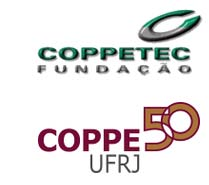
\includegraphics[width=40mm]{logo/coppetec50-logo.jpg}

\vfill%
\begin{center}
  {\GRANDE \raisebox{1.4ex}{} 
\includegraphics[width=80mm]{logo/projeto-EMMA-logo.jpg}} \\[10mm]
  %{\GRANDE \raisebox{1.4ex}{Projeto EMMA} } \\[10mm]
  {\Grande Relatório de Teste Experimental} \\[25mm]
  {\Grande Teste da Base Magnética} \\[20mm]
  {\large Usina Hidrelétrica de Jirau} \\[5mm]
  {\large 14 de Outurbo de 2015}
  \vfill%
  %{\Large \today} \\[8mm]
\end{center}

\newpage%
%---------------------------------------------------------------------
\pagestyle{fancy}%
\thispagestyle{fancy}%
\renewcommand{\headrulewidth}  {0.4pt}%
\renewcommand{\footrulewidth}  {0.4pt}%
\lhead{\vspace*{-6mm}
\includegraphics[width=30mm]{logo/lead-logo.jpg}}%
\chead{\vspace*{-6mm}\raisebox{1.7ex}{} 
\includegraphics[width=25mm]{logo/projeto-EMMA-logo.jpg}}%
%\chead{\vspace*{-6mm}\raisebox{1.7ex}{Projeto EMMA}}%
\rhead{\sf\thepage}%
\lfoot{Relatório de Teste Experimental}%
\cfoot{}%
\rfoot{\sf [\hours] \quad \today}%
%---------------------------------------------------------------------

%---------------------------------------------------------------------
%\tableofcontents

\newpage%
%---------------------------------------------------------------------



\section{Identificação}

%-----------------------------------------------------------------------
%
%   UFRJ  - Universidade Federal do Rio de Janeiro
%   COPPE - Coordenação dos Programas de Pós-graduação em Engenharia
%   PEE   - Programa de Engenharia Elétrica
%
%
%   Projeto EMMA - Metodologia para revestimento robótico de turbinas in situ
%
%   Identificação
%                                                         Ramon R. Costa
%                                                         07/jul/15, Rio
%-----------------------------------------------------------------------
%\section{Identificação}

\dado{Título}{
  EMMA - Metodologia para revestimento robótico de turbinas \textit{in situ} \\
}

\dado{Proponente}{
  Universidade Federal do Rio de Janeiro (UFRJ) \\[2mm]
  Fundação Coordenação de Projetos, Pesquisas e Estudos Tecnológicos (COPPETEC) \\
}

\dado{Contratante}{
  ESBR - Energia Sustentável do Brasil S.A. \\
}

\dado{Execução}{
  Grupo de Simulação e Controle em Automação e Robótica (GSCAR) \\
}

 \dado{Contrato}{
   Jirau 09-15 \\
 }

 \dado{P\&D ANEEL}{
   6631-0003/2015 \\
 }

%\dado{COPPETEC}{
%  N.D. \\
%}

\dado{Início}{
  01/03/2015 \\
}

\dado{Prazo}{
  14 meses \\
}

\dado{Orçamento}{
  R\$ 2.487.473,47 \\
}

\dado{Coordenador}{
  Ramon Romankevicius Costa \\
}

\dado{Gerente}{
  Breno Bellinati de Carvalho \\
}

%---------------------------------------------------------------------
\fim

\newpage%
%---------------------------------------------------------------------
\section{Teste Base Magnética}
\subsection{Visão geral}
Este teste visou testar a aplicabilidade da base magnética comercial do
fabricante MagTek, modelo PME-300, no ambiente da turbina. A base magnética
comercial é projetada para aderir a superfícies planas ou cilíndricas convexas.
No caso da turbina, as regiões testadas têm formatos variados, que dependendo da
orientação da base, podem ser cilíndricos côncavos ou convexos. As
superfícies também variam de material, tratamento superficial e pintura,
assim como limpeza e rugosidade.

Por esse motivo viu-se a necessidade de testar
\textit{in situ} a base magnética comercial e verificar os reais limites de
adesão magnética do equipamento.


%---------------------------------------------------------------------
\subsection{Equipamentos utilizados}
\begin{enumerate}
  \item Base Magnética 300 kgf;
  \item Plataforma de apoio;
  \item Alavanca 0,8 m;
  \item Dinamômetro 25 kgf
\end{enumerate} 

\begin{figure}[h!]
\centering
	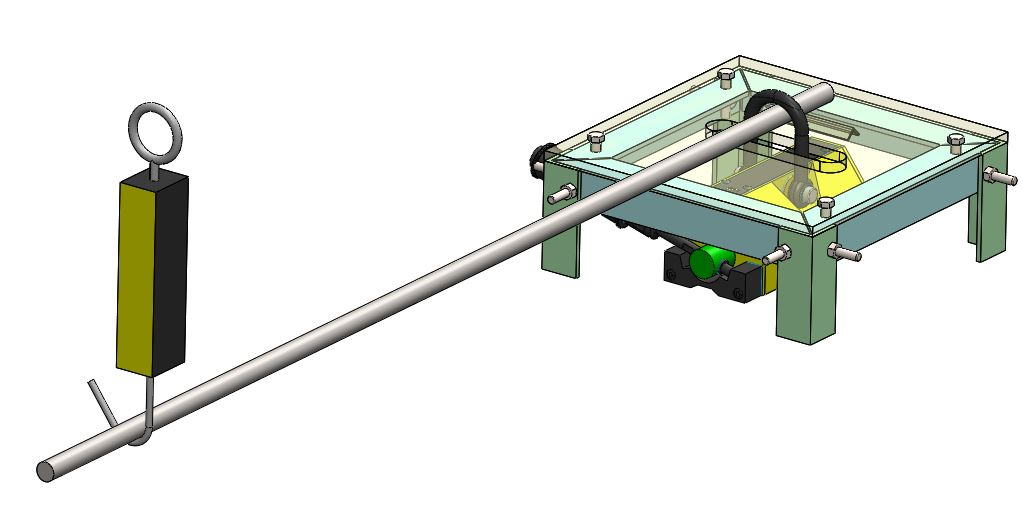
\includegraphics[width=0.9\columnwidth]{figs/conjunto_01.jpg}
	\caption{Conjunto de teste da base magnética}
	\label{fig::conjunto}
\end{figure}

\newpage
\subsection{Dados dos equipamentos}
\begin{description}
  \item[Base Magnética] \hfill
  \begin{itemize}
    \item Capacidade nominal: \\ [2ex]
	- no plano: 300 kgf \\
	- cilindro convexo: 150 kgf \\
	\item Capacidade máxima no plano: 960 kgf  
  \end{itemize}
  \item[Alavanca] \hfill \\
  De acordo com a figura~\ref{fig::esquematico}:
  \begin{itemize}
    \item Comprimento da alavanca: L
    \item Distância entre os apoios: d  	
  \end{itemize}
  Os valores de L e d foram medidos em cada resultado do teste e a razão
  L/d está indicada na tabela~\ref{table:1} da seção~\ref{sec::resultados}.
  \item[Dinamômetro] \hfill \\
  Capacidade máxima do dinamômetro: 25 kgf
\end{description}

\begin{figure}[h]
\centering
	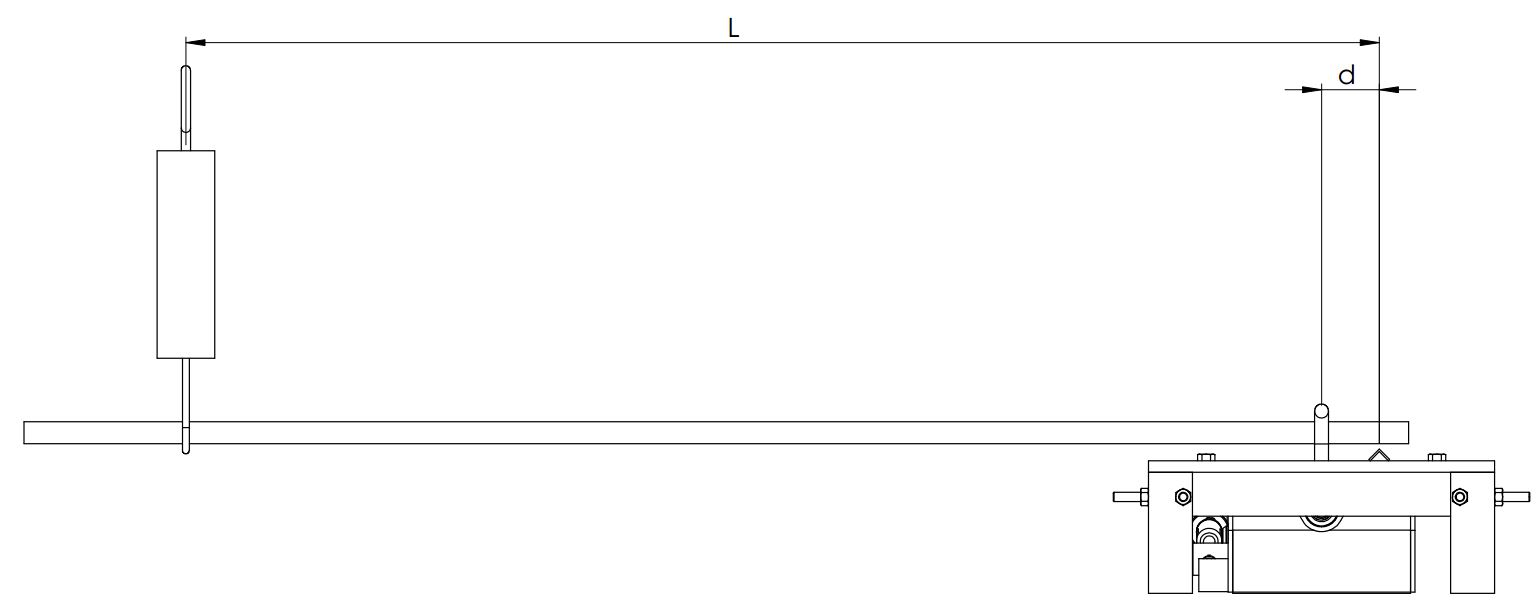
\includegraphics[width=0.9\columnwidth]{figs/esquematico.jpg}
	\caption{Esquemático da estrutura de teste com parâmetros de cálculo
	indicados}
	\label{fig::esquematico}
\end{figure}

%---------------------------------------------------------------------

\subsection{Cálculo da força magnética máxima}
A força magnética, em função da força medida no dinamômetro, está de acordo com
a equação~\ref{eq::fmag}:

\begin{equation} \label{eq::fmag}
F_{\text{mag}}=\frac{L}{d} F_{\text{din}}
\end{equation}


\subsection{Mapa de posicionamento} \label{sec::mapa}
Abaixo, apresenta-se um mapa esquemático das posições onde foram testadas a
adesão magnética da base.

\begin{figure}[h!]
\centering
	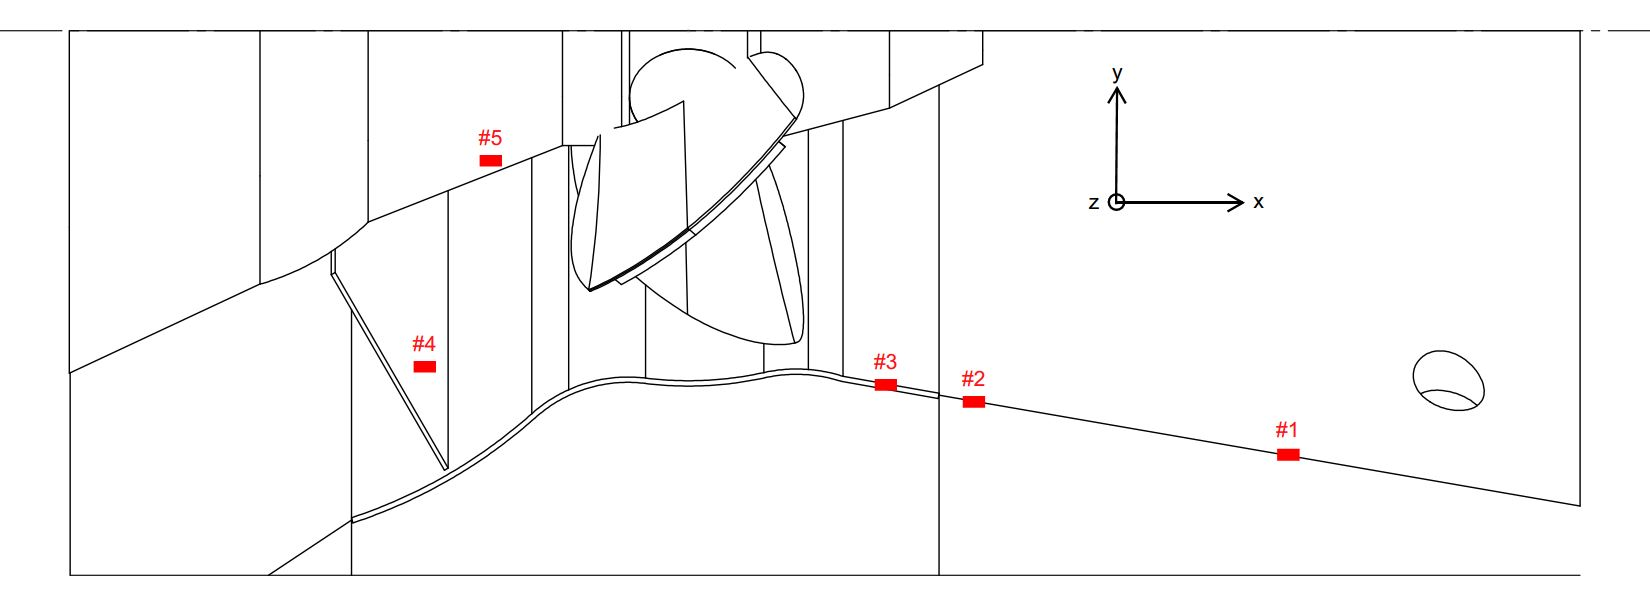
\includegraphics[width=0.8\columnwidth]{figs/mapa.jpg}
	\caption{Mapa esquemático de posições}
	\label{fig::mapa}
\end{figure}

\subsection{Procedimento} \label{sec::procedimento}
A adesão magnética foi testada nas posições indicadas no mapa esquemático da
seção~\ref{sec::mapa}. Para as posições 1 e 2 variou-se a orientação da base de
acordo com o eixo de coordenadas indicado na figura~\ref{fig::mapa}.

O procedimento de teste é o seguinte: 1) posiciona-se a base magnética; 2)
ativa-se o imã; 3) posiciona-se o apoio e a alavanca; 4) mede-se a distância
entre os apoios e o comprimento do braço de alavanca até o dinamômetro
(dimensões ''d'' e ''L''); 5) aplica-se gradualmente a carga na alavanca,
observando a indicação no dinamômetro, até que ocorra o primeiro dos dois casos:
a) o dinamômetro indica a carga máxima, ou b) a base magnética descola-se da
superfície; 6) anota-se o resultado.

\begin{figure}[h!]
\centering
	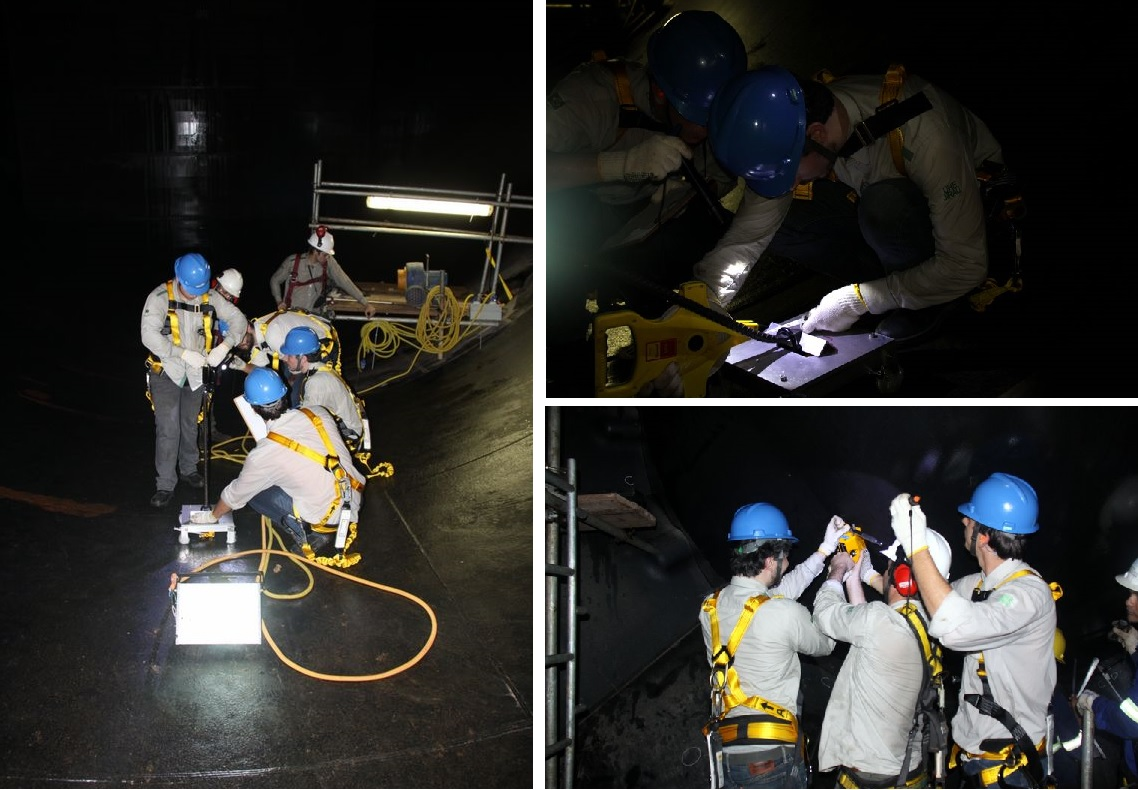
\includegraphics[width=0.5\columnwidth]{figs/fotos.jpg}
	\caption{Fotos durante o teste}
	\label{fig::fotos}
\end{figure}

\subsection{Resultados} \label{sec::resultados}
A tabela~\ref{table:1} apresenta o resultado do teste da base magnética nas
posições indicadas na seção~\ref{sec::mapa}.

\begin{table}[h!]
\centering
\begin{tabular}{||c c m{7em} m{4em} m{6em}||} 
 \hline
 Posição & Orientação & Força limite no dinamômetro (kgf) & L/d & Força
 magnética limite (kgf) \\  [0.5ex] 
 \hline\hline
 1 & x & 25 & 10,3 & 256 \\ 
 1 & x & 25 & 14,7 & 367 \\
 1 & x & 14 & 17,8 & 249 \\
 1 & z & 18 & 17,8 & 320 \\
 1 & x & 14 & 21,1 & 295 \\
 2 & z & 12 & 22,9 & 274 \\
 2 & x & 8,5 & 21,1 & 179 \\
 2 & xz 45º & 10 & 22,9 & 229 \\
 3 & x & 0 & 22,9 & 0 \\
 3 & z & 0 & 22,9 & 0 \\
 4 & n/a & n/a & n/a & n/a \\
 5 & n/a & n/a & n/a & n/a \\ [1ex]
 \hline
\end{tabular}
\caption{Resultados do teste experimental}
\label{table:1}
\end{table}

%---------------------------------------------------------------------

\subsection{Conclusões}
O teste possibilitou verificar a capacidade de adesão magnética para diferentes
posições, geometria de superfície e materiais no interior da turbina. O maior
valor encontrado, de 367 kgf, é superior até à capacidade de carga nominal para
superfícies planas indicada pelo fabricante. O menor valor encontrado, de 179
kgf ainda é superior ao valor máximo para superfícies cilíndricas, indicado pelo
fabricante.

Desta forma, considera-se que os valores nominais do equipamento fornecem uma
boa referência para o dimensionamento deste equipamento como base para uma
amarração robusta da solução mecânica do projeto.

A posição 3, de acordo com o mapa esquemático da seção~\ref{sec::mapa}, é uma
região composta por aço inoxidável e não forneceu adesão magnética. As posições
4 e 5 são respectivamente a superfície das paletas do distribuidor e a
superfície do rotor. Estas superfícies apresentaram boa adesão magnética, mas
não foi possível medir valores limite, pois tais posições não estavam previstas
no teste e o equipamento projetado não permitiria uma medição adequada.

\section{Teste sensor Faro Focus 3D X330}
\subsection{Visão Geral}
Este teste visou testar a aplicabilidade do sensor laser Faro Focus 3D X330 no
ambiente de trabalho da turbina. O dipositivo apresenta sensibilidade a
ambientes onde haja alta umidade, pois opera com um sistema de lentes e lasers e
caso apresente condensação em um desses componentes, o resultado final de
sensoriamento pode ser prejudicado. Por esse motivo foi necessário realizar
testes com o sistema para analisar a viabilidade técnica de se usar o sensor
para a aplicação do projeto EMMA. 


\subsection{Equipamentos utilizados}

\begin{enumerate}
\item Faro Focus 3D X330 
\item Tripé de apoio
\item Esferas Reflexivas com base magnética
\end{enumerate}

\begin{figure}[h!]
\centering
	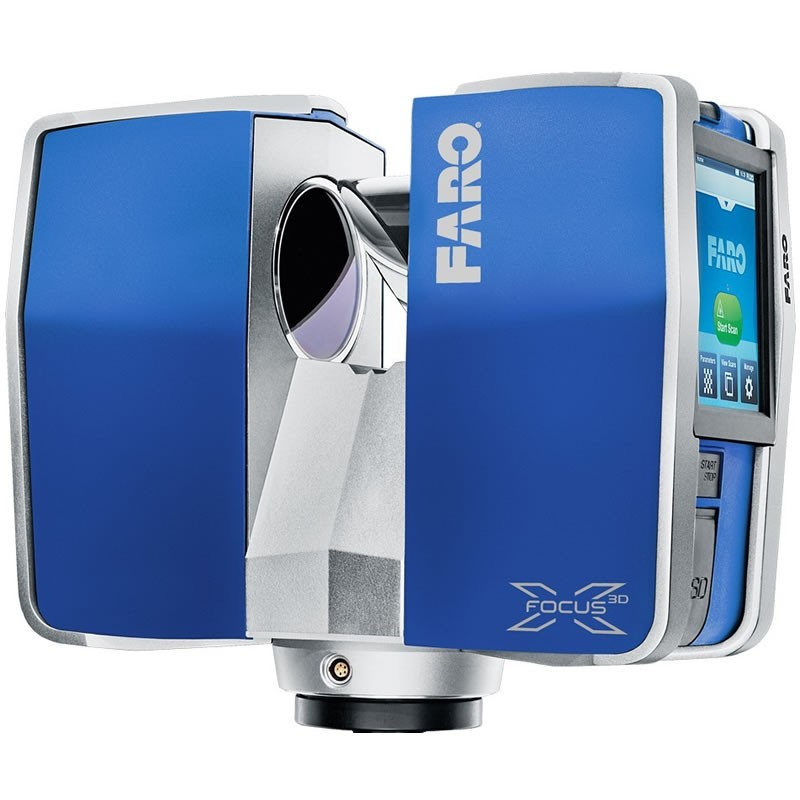
\includegraphics[width=0.4\columnwidth]{figs/faro/sensor}
	\caption{Sensor Faro Focus 3D X330.}
	\label{fig::sensor}
\end{figure}

\begin{figure}[h!]
\centering
	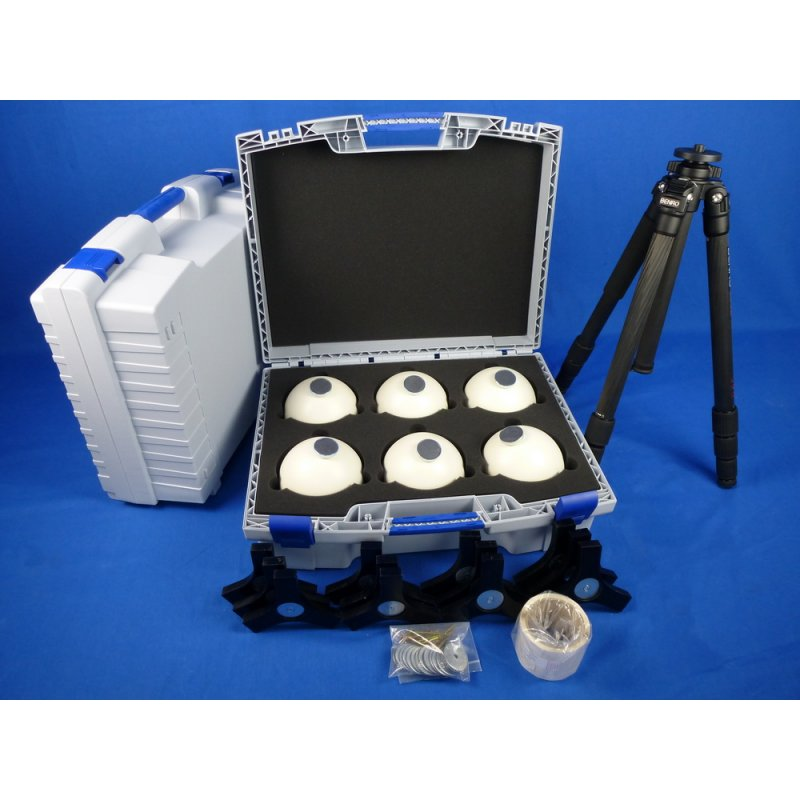
\includegraphics[width=0.5\columnwidth]{figs/faro/kit}
	\caption{Conjunto de esferas Reflexivas e tripé}
	\label{fig::kit}
\end{figure}


\subsection{Dados dos equipamentos}

\begin{itemize}
  \item Faro Focus 3D X300
  \begin{itemize}
    \item \textbf{Alcance:} 0,6 m - 330 m
    \item \textbf{Velocidade de medição (pts/seg.):}s 122.000 / 244.000 /
    488.000 / 976.000
    \item \textbf{Erro de alcance:} $\pm 2 mm$
    \item \textbf{Campo de visão vertical (vertical/horizontal):} 300$^o$ /
    360$^o$
    \item \textbf{Tamanho do passo (vertical/horizontal):} 0,009$^o$
    \item \textbf{GPS:} Receptor GPS integrados
    \item \textbf{Peso:} 5,2 kg
    \item \textbf{Temperatura ambiente:} $5^o - 40^o C$
    \item \textbf{Umidade:} Sem condensação
  \end{itemize}
\end{itemize}

\subsection{Procedimento}

\subsection{Resultados} 

\subsection{Conclusões}


%--------------------------------


%---------------------------------------------------------------------

\vspace{20mm}%
\parbox[t]{70mm}{
  \centering
  \includegraphics[width=65mm]{assinatura/assinatura-digital.jpg} \\[-4mm]
  \rule[2mm]{70mm}{0.1mm} \\
  \ramon \\[1mm]
  Coordenador do Projeto \\
}

\end{document}
